Das folgende Kapitel zeigt mögliche Anwendungen von Key Escrow Systemen und deren Alternativen für den Gebrauch von staatlichen Behördern, sowie in der Privatwirtschaft auf.
	
	\subsection{Staatlich}
		% Silvio
Die immer stärker werdenden kryptografischen Verfahren stellen die staatlichen Sicherheitsbehördern vor immer grössere Probleme. Die Anwendung von Verschlüsselung durch Straftäter erschwert die Arbeit der Sicherheutsbehörden enorm. \\
Nach terroristischen Anschlägen werden immer wieder Stimmen laut, welche die Einführung einer Möglichkeit zur Erleichterung der Entschlüsselung von Kommunikationsdaten fordern \cite{insideit} \cite{annabiselli} \cite{denning}. 
Dabei werden immer wieder die selbigen Themen angesprochen:

	\subsubsection{Erstellung eines Key Escrow Systemes}
Die Einführung eines Key Escrow Systemes wäre für jeden Geheimdienst wohl das höchste aller Gefühle. Allerdings hat ein staatliches Key Escrow System politisch einen sehr schweren Standpunkt. Dies liegt vor allem daran, dass ein solches System zu einem gewaltigen Verlust, wenn nicht gerade eine totale Aufgabe der Privatsphäre zur Folge hätte und die Gesellschaft kaum mit einer so drastischen Massnahme einverstanden wäre.\cite {insideit} \\
Fraglich wäre auch der Nutzen des Sytems im Hinsicht auf grössere kriminelle Organisationen. Zu glauben, dass alle Kriminellen Verschlüsselungstools benutzen würden, für welche der Schlüssel im Escrow System hinterlegt ist wäre sehr fraglich. Beispielsweise hat die Terrororganisation Al-Qaida von der Organisation nahestehenden Kryptologen ein eigenes Verschlüsselungssystem entwickeln lassen \cite{denning}. Dass es sich dabei nicht um einen Einzelfall handelt, lasst sich auch stark annehmen.
	
	\subsubsection{Hinterlegung von verwendeten Verschlüsselungsalgorithmen}
Eine nicht so schwerwiegende Alternative zu Key Escrow wäre die Hinterlegung des Verschlüsselungsverfahrens ohne Hinterlegung des verwendeten kryptografischen Schlüssels. Diese Hinterlegung sollte zum Nutzen haben, dass den Strafverfolgungsbehörden die Arbeit etwas erleichtert würde. Dies hätte allerdings auch nur dann einen Nutzen, wenn nur schwächere oder Algorithmen mit einer Sicherheitslücke verwendet werden dürfen. Diese Lücken wären somit auch ein Eigentor für die Sicherheitsbehörden, da sie somit Kriminellen eine weiter Angriffsfläche auf die Bürger bieten würden. \cite{adminch} % KP. 7.3.

	
	\subsubsection{Verbot von alternativen Verschlüsselung}
Die Einführung eines Escrow Systemes oder die Einführung einer Hinterlegungspflicht für Algorithmen würde auch dazu führen, dass die Gegenseite, das heisst die Verwendung nicht hinterlegter Schlüssel / Algorithmen, verboten werden müsste. Auf der einen Seite wäre ein solches Verbot sehr schwer durchzusetzten, geschweige überhaupt zu kontrollieren, auf der andern Seite wäre es von der Strafnorm her auch kaum möglich, eine genug hohe Maximalstrafe ansetzen zu können, um grössere kriminelle Organisationen von der illegalen Verwendung der Verschlüsselung abzuwenden. \cite{adminch} \\ %KP 7.3.
Zudem wäre ein solches Verbot auch nur dann vernünftig brauchbar und durchsetzbar, wenn es von der internationalen Gemeinschaft getragen und somit in allen Ländern durchgesetzt würde \cite{denning}. Da der Internationale Weg in Sache Verschlüsselungspolitik in eine andere Richtung weht, zeigt sich darin, dass sich einige Länder, welche in den neunziger Jahren die Kryptografie noch eingeschränkt hatten, in Richtung einer offenen Kryptografiepolitik bewegen. \cite{clipperchip} \cite{adminch} \\ % 7.2.3
Eine Einführung eines solchen Verbotes würde einen Staat interational stark ins Abseits setzten und das Verbot wäre somit auch kaum duchsetzbar.
		
	\subsection{Firmenintern}
Das nachfolgende Kapitel gibt einen Überblick über die Problembereiche beim Key Management von Firmen und zeigt auf, inwiefern Hintertüren (z.B. für staatliche Eingriffe) in Software eingebaut werden.

	\subsubsection{Key Management Systeme (KMS)}	
Geschäftskritische Daten sollten immer verschlüsselt werden. Um den Überblick über die verwendeten Schlüssel zu bewahren, können Key Management Systeme (KMS) eingesetzt. Diese stellen dabei ein firmeninternes Escrow-System dar.
Mit diesen Systemen lassen sich nebst der Datenverschlüsselung folgende Dinge realisieren:
\begin{enumerate}
	\item Datensicherheit durch Verschlüsselung gewährleisten
	\item Schlüssel können zentral verwaltet werden (Firma behält Überblick über verwendete Schlüssel)
	\item Entschlüsseln von Geschäftsdaten von Mitarbeitenden bei Tod, Abwesenheit oder Arbeitsverweigerung
  	\item Überwachung von Mitarbeitern
\end{enumerate}
Punkt 3 zeigt auf, welche Problematiken durch starke Verschlüsselung entstehen können. Werden die Daten eines Mitarbeiters durch einen eindeutigen privaten Schlüssel des Mitarbeiters verschlüsselt, hat nur der Mitarbeiter Zugriff auf die Daten. Ohne den Mitarbeiter selber kann das Geschäft die Daten nicht auslesen. Fällt der Mitarbeiter aus, können die Daten nicht wiederhergestellt werden. Wird der Schlüssel jedoch zusätzlich bei einem Treuhänder oder firmenintern hinterlegt, sind die Daten trotzdem wieder dechiffrierbar.
Die staatliche Key Escrow Idee wird meistens abgelehnt (\textit{Schnüffelstaat}). In diesem Beispiel wurde jedoch aufgezeigt, dass Key Escrow nicht direkt mit Spionage und Totalüberwachung gleichgesetzt werden sollte.

	\subsubsection{Key Escrow in Software am Beispiel des Windows BitLocker}
Der Windows BitLocker zeigt auf, wie Key Escrow in moderner Software implementiert werden kann. Der BitLocker ist eine Festplatten-Verschlüsselungssoftware von Microsoft, welcher standardmässig mit Windows mitgeliefert wird. \\
Mittels einem Recovery Key kann die Festplatte wieder entschlüsselt werden. Es stellt sich nun die Frage, \textit{wo} dieser Recovery Key gespeichert werden soll. Der BitLocker stellt dabei folgende Optionen zur Verfügung:

\begin{figure}[H]
	\centering
	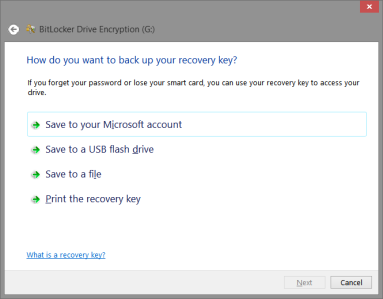
\includegraphics[width=.8\textwidth]{bitlocker-options.png}
	\caption{Wo soll der Recovery Key gespeichert werden?}
	{\cite{bitlocker}}
	\label{fig:clipper-chip}
\end{figure}
\textbf{Save to your Microsoft account} wirft dabei bezüglich Sicherheit Fragen auf.
\begin{itemize}
	\item Kann der Schlüssel immer wieder abgerufen werden?
	\item Wie lange wird der Schlüssel gespeichert?
	\item Wer erhält sonst noch Zugriff auf den erstellten Schlüssel?
\end{itemize}
Sobald man Daten in die Cloud lädt, verliert man die Hoheit über die Daten. Gesunder Menschenverstand lässt vermuten, dass die Daten vertraulich behandelt werden. Aufgrund der Snowden-Enthüllungen ist jedoch eine gesunde Portion Skepsis gegenüber Cloud-Diensten sicherlich nicht unangebracht.\\
Der BitLocker zeigt anhand eines einfachen Beispiel, wie schnell man die Hoheit über seine Schlüssel verlieren kann. Es ist schwierig bis unmöglich festzustellen inwiefern Software-Hersteller (insbesondere die Grossen wie Microsoft, Apple oder Google) Hintertüren für Staat und Geheimdienste in ihre Software eingebaut haben. Letzten Endes muss jeder Benutzer für sich entscheiden, inwiefern er den Cloud-Diensten vertraut und welche Informationen er in ihnen speichert.

	\subsection{Clipper Chip / Escrowed Encription Standard (EES)} \label{ssec:clipperchip}
\begin{figure}[H]
	\centering
	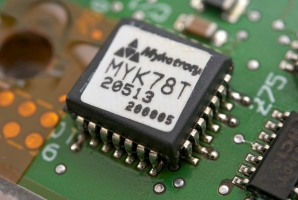
\includegraphics[width=.8\textwidth]{clipper-chip.jpg}
	\caption{MYK-78 Clipper Chip (1993)}
	\label{fig:clipper-chip}
\end{figure}
Ein exemplarisches Beispiel für staatlich erzwungenes Key Escrow ist der sogenannte Clipper Chip, welcher im Jahre 1993 durch die US-Behörden vorgestellt wurde und von der NSA entwickelt wurde.\\
Der Clipper Chip gehört zum Escrowed Encryption Standard (EES), welche hardwaremässige Verschlüsselung mit einer staatlich eingebauten Hintertür bietet. Die Behörden konnten die Verschlüsselungsmechanismen für jeden Clipper Chip rückgängig machen und so an die ursprünglichen Daten kommen. \\
Eingesetzt werden sollte der Chip in staatlicher und privater Kommunikation. Der Haupteinsatzzweck lag bei verschlüsselter Telefonie. \cite{ees}\\
Entworfen wurde der Chip von Mykrotronx, hergestellt von VLSI Technology Inc. \\

	\subsubsection{Funktionsweise und Aufbau}
Der Clipper Chip verwendet zur Verschlüsselung den Skipjack-Verschlüsselungsalgorithmus welcher dem DES-Algorithmus ähnelt. Entwickelt wurde Skipjack von der NSA und wurde bis zur Veröffentlichung im Jahre 1998 unter Verschluss gehalten. Nur wenige zivile Experten erhielten Einsicht in den Sourcecode. \cite{ees}\\
Zentrales Element der nach EES verschlüsselten Kommunikation ist das \textit{Law Enforcement Access Field (LEAF)} welches bei der Kommunikation zwischen zwei Geräten mitgeschickt wird.\\
Der Aufbau des 128bit grossen LEAF sieht wie folg aus:
\begin{itemize}
	\item \textbf{Unit ID} (32 bit): Eindeutige ID pro Chip (bei Herstellung vergeben)
	\item \textbf{Encrypted Session Key} (80 bit): Session Key, verschlüsselt durch gerätespezifischen Unit Key
	\item \textbf{Checksum} (16 bit): Zur Fehlerüberprüfung
\end{itemize}
Wünschen zwei EES-fähige Geräte eine verschlüsselte Kommunikation, handeln diese als erstes einen eindeutigen, temporären \textit{Session Key} aus. Dieser wird mittels eindeutigem, gerätespezifischen Unit Key verschlüsselt. Das somit generierte LEAF wird zusätzlich mit einem \textit{Family Key} verschlüsselt, welcher pro EES-Gerätefamilie eindeutig ist.\\
Nachfolgend werden die verwendeten Keys zusammengefasst:
\begin{itemize}
	\item \textbf{Unit Key}: Eindeutig pro Clipper Chip.
	\item \textbf{Session Key}: Temporärer Key für eine Session. Wird bei Kommunikationsbeginn von den beiden Geräten ausgehandelt. 
	\item \textbf{Family Key}: Eindeutig pro EES-Gerätefamilie
\end{itemize}
\begin{figure}[H]
	\centering
	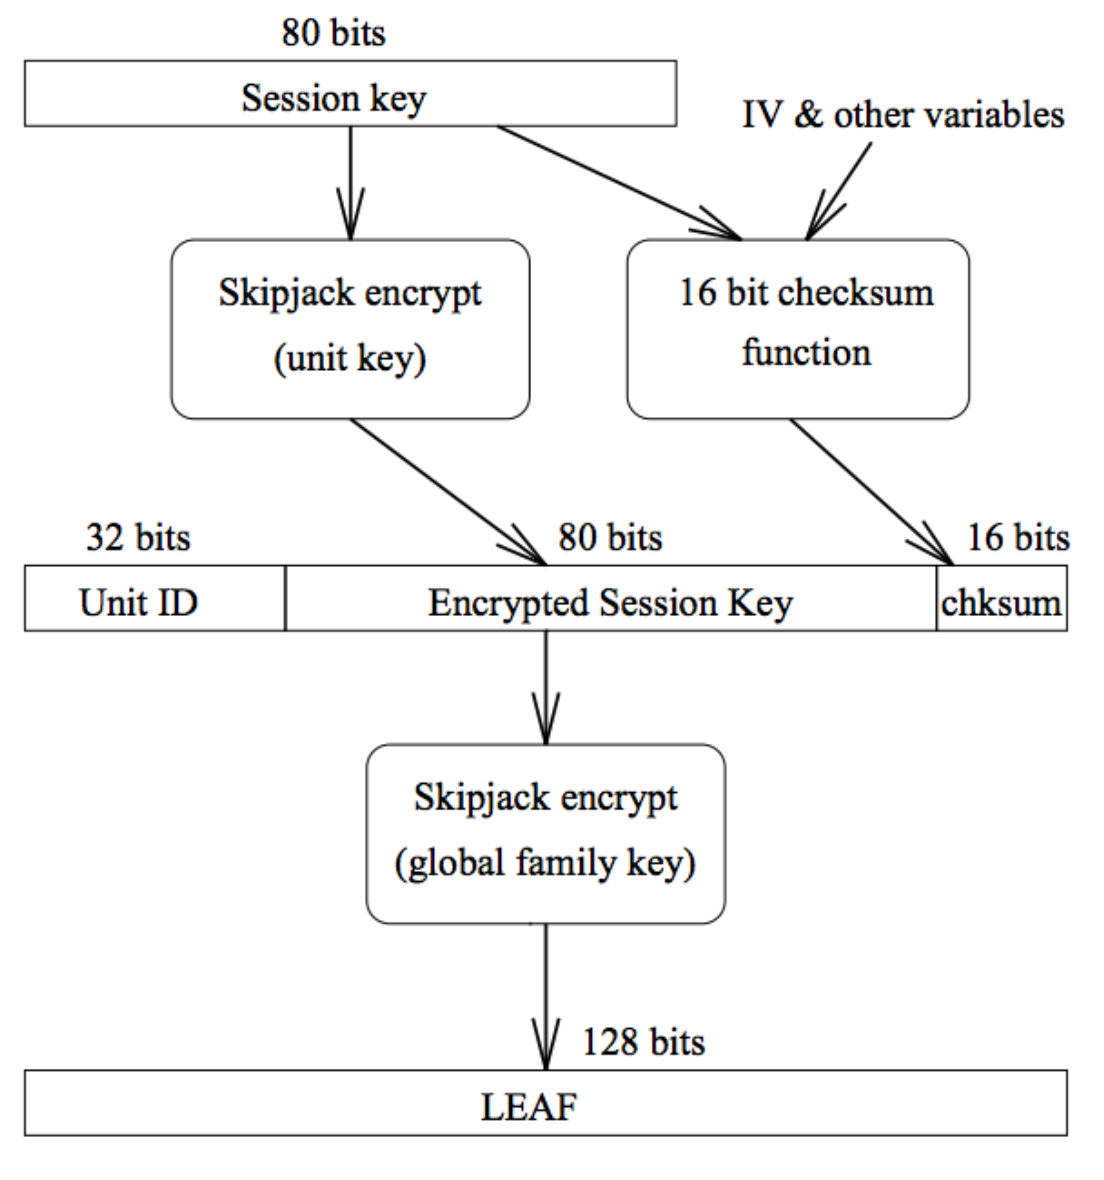
\includegraphics[width=.8\textwidth]
		{leaf-aufbau.png}
	\caption{Aufbau LEAF gemäss}
	{\cite{ees}}
	\label{fig:leaf-aufbau}
\end{figure}
Der \textit{Unit Key} wird dabei aufgespalten und bei zwei voneinander getrennten nationalen Behörden gespeichert. Dies dient dazu, Amtsmissbrauch einzudämmen. Soll aufgrund einer richterlichen Anordnung eine verschlüsselte Kommunikation abgehört werden, wird das LEAF mittels \textit{Family Key} dechiffriert. Daraus kann die Unit ID gewonnen werden. Mit der ID werden bei den zwei Behörden die beiden Teile des \textit{Unit Key} angefordert und zusammengefügt. Daraus kann danach der \textit{Session Key} und aus diesem wiederum die verschlüsselten Daten entschlüsselt werden.
\begin{figure}[H]
	\centering
	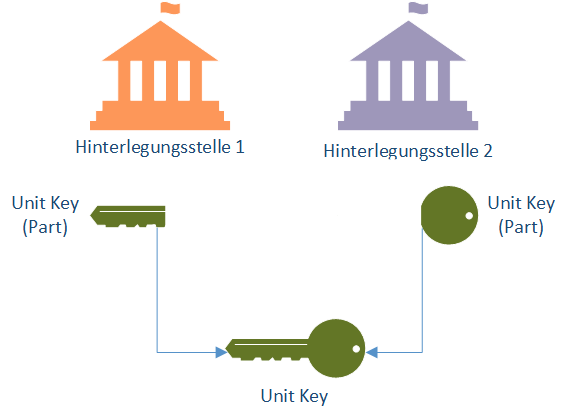
\includegraphics[width=.8\textwidth]
		{EES-Hinterlegungsstelle.png}
	\caption{Der Unit Key wird für den Schutz vor Amtsmissbrauch gesplittet an zwei Stellen hinterlegt. Beide Teile fügen sich zum gesamten Key zusammen.}
	\label{fig:clipper-chip-in-escrow}
\end{figure}

	\subsubsection{Technische Schwachstelle}
Im Jahr 1994 veröffentlichte Matt Blaze von AT\& T ein Paper, in dem er eine wesentliche Schwachstelle des Systemes aufzeigte. Wie in Abbildung \ref{fig:leaf-aufbau} zu sehen ist, wird dem LEAF eine Prüfsumme in Form eines Hash mitgegeben. Diese Prüfsumme wird benötigt, damit Manipulationen des LEAF ausgeschlossen werden können. Stimmt die Prüfsumme nicht mit dem errechneten Hash des LEAF überein, werden die gesendeten Nachrichten vom Clipper Chip nicht dechiffriert. \\
Forschungen von Matt Blaze zeigen, dass dabei die Länge des Keys (16bit) nicht genügend gross ist, um einer \textit{Brute Force Attacke} standzuhalten. \cite{ees}
Einem Angreifer wird es also ermöglicht, denselben Hash-Wert für ein LEAF mit einem gefälschten Session Key zu erzeugen. Die Escrow-Behörde erhält somit ein vermeintlich gültiges LEAF, beim aufschlüsseln jedoch einen gefälschten Session Key, mit welchem sich die versendeten Nachrichten nicht dechiffrieren lassen.

	\subsubsection{Das Ende des Clipper Chip}
Die Idee Clipper Chips kam bei der Bevölkerung nicht gut an. \textit{"You don't want to buy a set of car keys from a guy who specializes in stealing cars"}, kommentierte Marc Rotenberg vom Electronic Privacy Information Center die Pläne der Behörden. \cite{ees_nytimes}\\
Spätestens im Jahr 1996 wurde der Clipper Chip irrelevant und wird seither nicht mehr weiter produziert. Parallel zum Clipper Chip wurden starke, frei verfügbare Datenverschlüsselungsmechanismen wie etwa PGP (Pretty Good Privacy) auf den Markt gebracht, welche die Idee eines staatlich kontrollierten Escrow-Systems verdrängten. Die Bevölkerung und Hersteller trauten den Behörden zu wenig.

	\subsection{Recovery Agents und Trusted Third Parties}
Bei Key Escrow handelt es sich um ein Verfahren um Schlüssel für den späteren Gebrauch zu hinterlegen. Key Recovery ist der Prozess der Schlüssel anhand bestehender Daten rekonstruiert.
\\
Falls Key Recovery, beziehungsweise Key Escrow, von zwei Parteien erwünscht ist, wird meist eine Trusted Third Party als unabhängige Kontroll- und Aufsichtsinstanz hinzugezogen.
\\
Die ausführende Instanz für Key Escrow und Key Recovery ist als Teil einer Trusted Thir Party der Recovery Agent.
		\subsubsection{Recovery Agent als Man in the Middle bei symmetrisch verschlüsselter Kommunikation}
Die beiden nachfolgenden Abbildungen illustrieren eine einfache funktionsweise eines Recovery Agent gemäss Belser \cite{isss}. Die Architektur ähnelt der des Clipper Chip (siehe Kapitel \ref{ssec:clipperchip})
\begin{figure}[H]
	\centering
	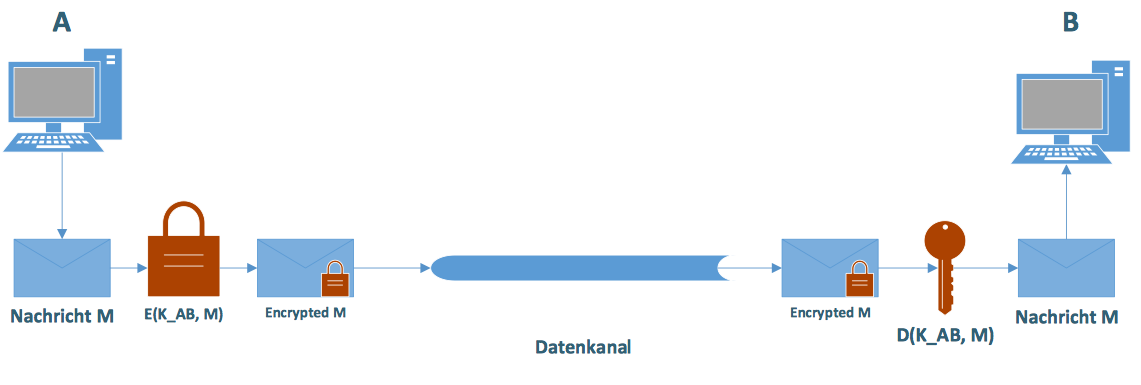
\includegraphics[width=\textwidth]
		{recovery-agent-aufbau.png}
	\caption{Symmetrische Verschlüsselung einer Kommunikation}
	\label{fig:recovery-agent-aufbau}
\end{figure}
In Abbildung \ref{fig:recovery-agent-aufbau} werden zwei kommunizierende Computer dargestellt. \textit{A} nimmt die Rolle des Senders und \textit{B} die Rolle des Empfängers ein. Sie nutzen zur Verschlüsselung der Nachricht ein symmetrisches Chiffrierverfahren. Der genutzte Schlüssel $K_{AB}$ wurde bereits ausgetauscht. \textit{A} erstellt die Nachricht $M$ und chiffriert sie mittels $E(K_{AB},M)=M_{C}$. Die chriffrierte Nachricht $M_{C}$ wird über den Datenkanal übertragen und von \textit{B} empfangen. Nach Dechiffrierung mittels $D(K_{AB},M_{C})=M$ kann die Nachricht $M$ von \textit{B} weiterverarbeitet werden.
\begin{figure}[H]
	\centering
	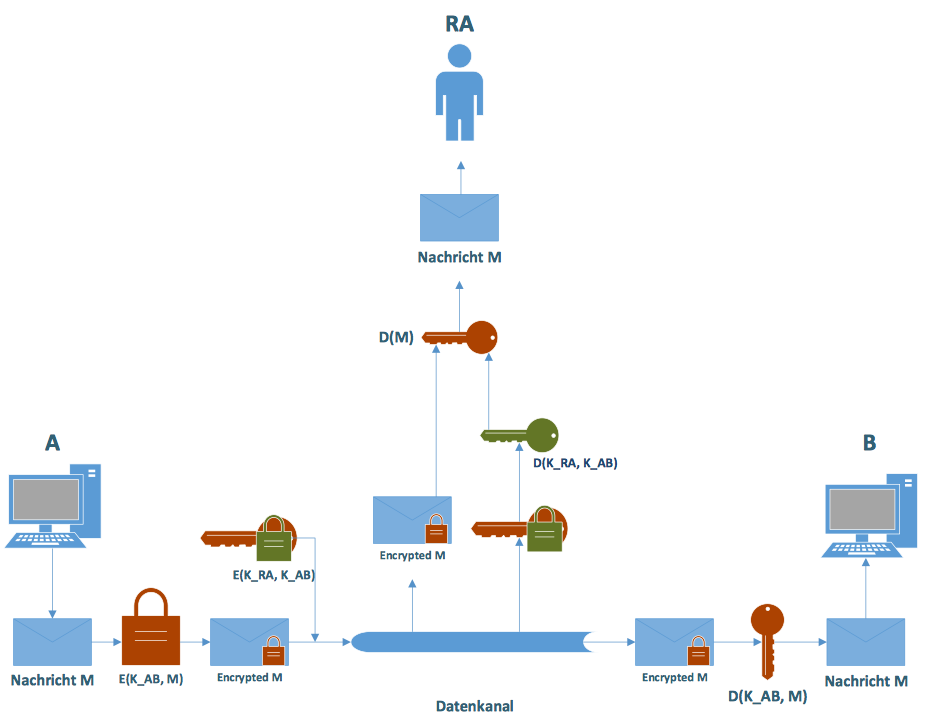
\includegraphics[width=.8\textwidth]
		{recovery-agent-mitm.png}
	\caption{Recovery Agent als Man in the Middle}
	\label{fig:recovery-agent-mitm}
\end{figure}
Abbildung \ref{fig:recovery-agent-mitm} erweitert die symmetrisch verschlüsselte Kommunikation von \textit{A} und \textit{B} mit einem Recovery Agenten \textit{RA}.
\\
Dieser besitzt ebenfalls einen Schlüssel $K_{RA}$. Beim Senden der Nachricht $M$ wird ebenfalls der chiffrierte Schlüssel $E(K_{RA},K_{AB})=C_{K_{AB}}$ von \textit{A} übertragen. Der Recovery Agent \textit{RA} hört die chiffrierte Nachricht $M_{C}$ und den chiffrierten Schlüssel $C_{K_{AB}}$ vom Datenkanal ab. Er dechiffriert den Schlüssel von \textit{A} und \textit{B} mittels $D(K_{RA}, C_{K_{AB}})=K_{AB}$ und kann somit auch die chiffrierte Nachricht $M_{C}$ dechiffrieren.
